\section{Case description} \label{ch:case description}

In this project, we are going to focus on the Universal Robot, UR5 which is an industrial manipulator.\\
The UR5 is going to assist in the balancing and leak test of a L40 rotor see \ref{fig:rotor} that is being produced at Grundfos. The L40 rotor arrives at the work-cell via a conveyor belt. The rotor has to go through a balancing machine, where the rotor is placed in a drawer. It must then pass a visual inspection performed by an employee, before it is sent to the leak testing machine.\\
The leak testing machine can test two rotors per load, and when the leak test is comeplete, the machine will give a signal if the rotor has passed the test or not. The rotor will then be placed in an engraving machine which prints an ID onto the rotor. It will then moved to the output pallet, which will be moved to another location, and replaced with a new pallet by an employee.\\ 
After being processed in the leak testing machine, the rotors can be placed on a queue table, until the engraving machine is ready. Each rotor must undergo this entire process in 26 seconds or less.\\


\begin{figure}
    \centering
    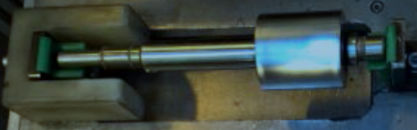
\includegraphics[width=9cm]{InitialProblemstatement/Case/rotorlille.PNG}
    \caption{The L40 rotor \cite{Case}}
    \label{fig:rotor}
\end{figure}



